%----------------------------------------------------------------------------------------
% hllc_rstates.tex
%----------------------------------------------------------------------------------------

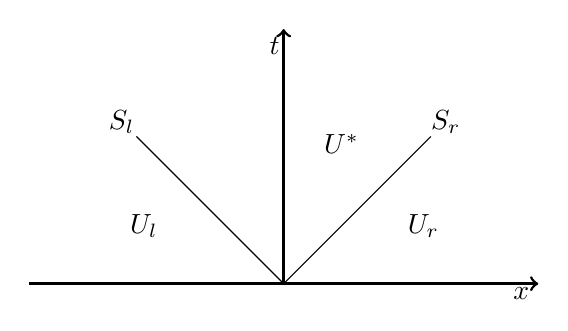
\begin{tikzpicture}[scale = {0.0125\linewidth},inner sep = 1pt]
%% \begin{tikzpicture}[scale = {0.015\linewidth},inner sep = 1pt]
%% \tikzstyle{every node} = [draw,circle,fill=gray!30];
%% \draw (-1.5,0.0) circle (0.8);
%% \draw[<->,line width=1pt] (0,1) node[right]{\;$t$}|-(1,0) node[below]{$m$};
\draw[line width=1pt] (0,0.7) node[left]{$t$}|-(0.7,0) node[below]{$x$};
\draw[->,line width=1pt] (0.7,0)--(0.75,0);
\draw[->,line width=1pt] (0,0.7)--(0,0.75);  
\draw[line width=1pt] (-0,0)--(-0.75,0);
\node[draw=white] (sr) at (0.47730,0.47730) {$S_r$};
%% \node[draw=white] (cd) at (0.058830,0.67243) {$S_m$};
\node[draw=white] (sl) at (-0.47730,0.47730) {$S_l$};

\node[draw=white] (ur) at (0.41159,0.17049) {$\mbf{U}_{r}$};
\node[draw=white] (usr) at (0.17049,0.41159) {$\mbf{U}^*$};
%% \node[draw=white] (usl) at (-0.17049,0.41159) {$\mbf{U}^*_{l}$};
\node[draw=white] (ul) at (-0.41159,0.17049) {$\mbf{U}_{l}$};

\draw (0,0) -- (sr);  
%% \draw (0,0) -- (cd);  
\draw (0,0) -- (sl);  

\end{tikzpicture}
